\chapter{MASSIVE Language}
\label{usecase}

In this report we illustrates how we designed and implemented the agent oriented language, MASSIVE. During this chapter we demonstrates a working simulation with a use case, and compare the agent oriented language to Object Oriented Code (C\#). Furthermore we discuss the advantages and disadvantages of the MASSIVE language. 

\section{Use Case}
In this use case we demonstrate how to write a mini-game in our language, how to compile it and how to play it. \\
 \\
The first thing one needs to do is to write some MASSIVE code. In the following code example are examples of MASSIVE code, however there are features of the langauge that are not being used in this example. For a full code referernce please check \ref{uftml}. In the example two teams are created called "Disco" and "Kman", agents are added to them and at the end a simple action pattern is defined, later to be used when running the simulation.

\begin{source}{MASSIVE code example}{}

/* Initializes the game with the properties
Maximum Units = 400 */
Main ( 400 )
{	
	
	// Creates team Disco.
	new team teamDisco("Disco", "#FF6600");
	num totalDiscos = 10;
	for ( num i = 0; i < totalDiscos; i = i + 1)
	{
		num a = 0;
		if ( i < totalDiscos-1 )
		{
			a = 1;
		}
		else
		{
			a = 21-totalDiscos;
		}
		
		new Agent newAgent("Stue", a);
		teamDisco.add(newAgent);
	}
	
	new team teamKman("Kman", "#660000");
	new squad squadNabs("noobs");
	new squad squadRevo("Revolution");
	
	for(num i = 0; i < 4; i = i + 1)
	{
		num a = 0;
		if(i =< 1)
		{
			a = 2;
		}
		if(i >= 2)
		{
			a = 8;
		}
		
		new Agent newAgent("Kman", a);
		teamKman.add(newAgent);
		
		if (i <= 1)
		{
			squadNabs.add(newAgent);
		}
		if (i => 2)
		{
			squadRevo.add(newAgent);
		}
	}
	
	// Moves used in the actionPatterns.
	string moveUp = "unit move up";
	string moveDown = "unit move down";
	string moveLeft = "unit move left";
	string moveRight = "unit move right";
	
	// Creates the action pattern Patrol Low.
	// Patrols the lower part of the game area.
	new actionpattern patrolLow("PatrolLow");
	patrolLow.add(moveUp);
	patrolLow.add("unit move 25,24");
	patrolLow.add(moveUp);
	patrolLow.add("unit move 0,23");
	patrolLow.add(moveDown);
	
}
\end{source}
When compiling this code the compiler warns that there are unused variable (see \ref{fig:compiler}). We will disregard this for the purpose of this use case, however, if there were serious faults in the code the compiler would warn you the same manner and maybe even refuse to compile if the faults were serious enough.

\begin{figure}[h]%
\begin{center}
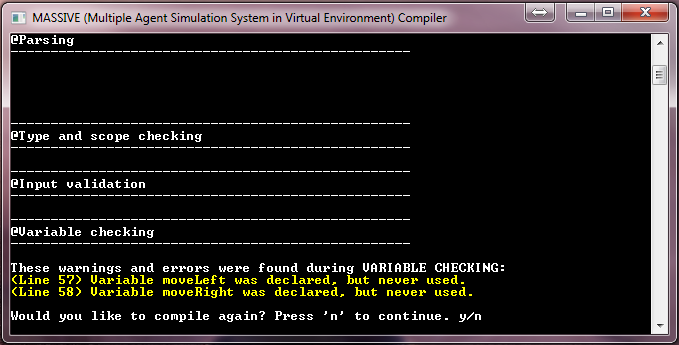
\includegraphics[width=\columnwidth]{Images/compiler.png}%
\end{center}
\caption{The MASSIVE compiler warning of unused variables.}%
\label{fig:compiler}%
\end{figure}

The compiler will happily compile the code again if that option is selected, which provides the programmer with an easy way of correcting erroneous code. After a succesfull compilation a file named "MASSIVECode.cs"and "MASSIVECode.exe" will have been created. The only purpose of creating the cs-file is allowing the programmer to have a look at the code our compiler generates. The cs-file will have been compiled into the exe-file wich is run automatically. This exe-file creates the actual data output in XML format, which is then run by the MASSIVE simulator, and the user of the simulator is given a choice of how large the game grid will be (see \ref{fig:game_promt}).

\begin{figure}[h]%
\begin{center}
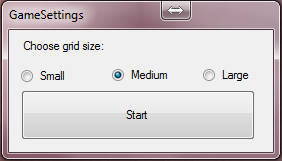
\includegraphics[width=\columnwidth]{images/massive_dialog.png}%
\end{center}
\caption{Choosing the size of the game-grid}%
\label{fig:game_promt}%
\end{figure}

Upon choosing "large", the user will bee presented with the actual simulation (see \ref{fig:runninggame}). Here he will have the oppertunity to instruct the agents to use the action pattern defined in the previous code example, as shown in \ref{fig:runninggame}.

\begin{figure}%
\begin{center}
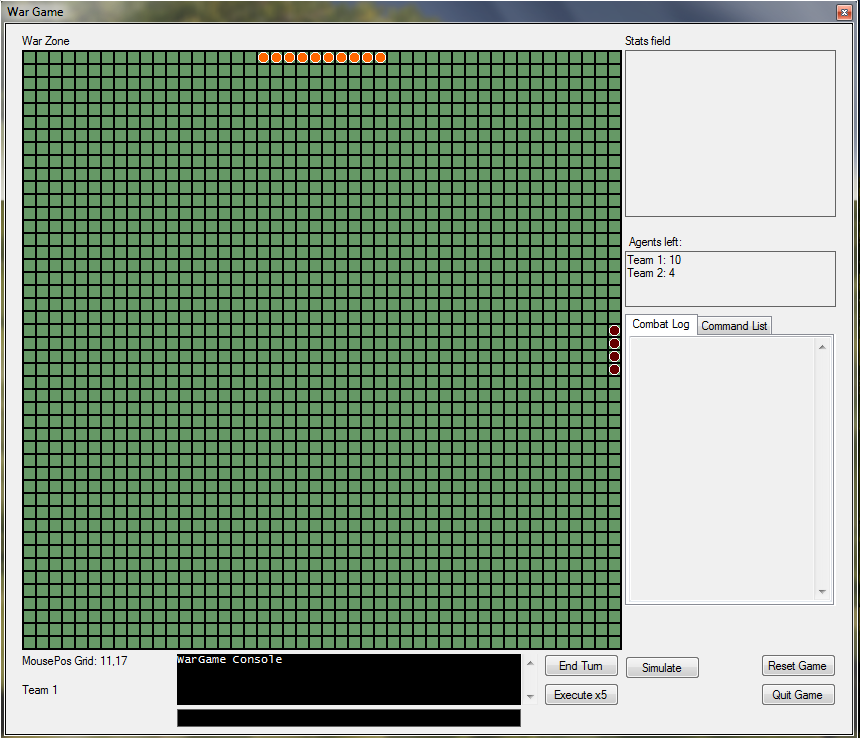
\includegraphics[width=\columnwidth]{Images/massive_small.png}%
\end{center}
\caption{The simulation running with the input instructing som of the agents to use an actionpattern}%
\label{fig:runninggame}%
\end{figure}

At this point the user is presented with a choice; He can either press "Simulate" to let the simulation run to an end without any interaction, or he can choose to run the game turn-by-turn and control the agents as the game progresses. We see the result of this simulation in \ref{fig:winner}.

\begin{figure}%
\begin{center}
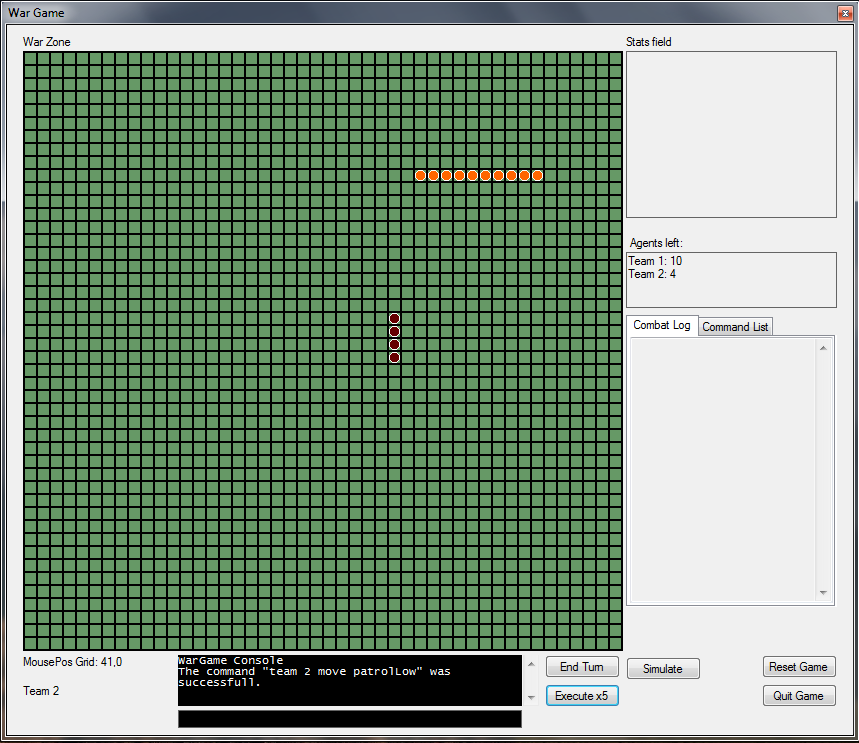
\includegraphics[width=\columnwidth]{Images/massive_patrollow.png}%
\end{center}
\caption{The result of the use case simulation in MASSIVE}%
\label{fig:winner}%
\end{figure}

\section{Comparison}
\indent This section is about how to build a multi agent wargame using C\# compared to our own language MASSIVE. We will take a look on some of the pros and cons by using C\#  aswell as the pros and cons using MASSIVE. We will then compare C\# and MASSIVE to examine which language is the best to build a multi agent wargame.

\section{C\#}
We have decided to compare MASSIVE with C\# which is an object orientated language(OOP). We decided to use C\# to compare with because both our compile and enviroment are written in this language. C\# do not have built in multi agent orientated functions or enviroments, which means it is required for the programmer to build the multi agent wargame from scratch. To build a basic multi agent wargame in C\# you need to make constructors for agent and teams, furthermore you will also need to create functions for agents and teams, which could be movement and attack functions. At last you would need to create an enviroment to simulate a wargame. However building a multi agent wargame in C\# enables you to create all the features you want in a wargame simulation.\\

Pros
\begin{itemize}
	\item No limits, you can create all the features you want.\\
\end{itemize}

Cons
\begin{itemize}
	\item No existing multi agent enviroment.
	\item No existing multi agent types.
	\item No existing multi agent functions.
\end{itemize}

\section{MASSIVE}
MASSIVE is a agent orientated language(AOL) which contains premade enviroment and functions for creating agents, squads, teams, and actionpatterns, which means that you do not have to build these yourself and it is therefore relative fast to simulate a wargame. You cannot declare new functions in MASSIVE which limit you to only use the built in functions. The types and functions of MASSIVE are not case sensitve, so you do not need to worry about writing in upper or lower case.\\

Pros
\begin{itemize}
	\item Relative fast to simulate a wargame.
  \item	Premade enviroment.
	\item Premade types for agent, squad, team, actionpattern.
	\item Types and functions are not case sensitive.
\end{itemize}

Cons
\begin{itemize}
	\item Limited to the languages functions.
\end{itemize}

%Good and abd things about MASSIVE
%Why is our MASSIVE better than OOP. 
\section{C\# vs MASSIVE}
We will in this section compare a C\# code example to the MASSIVE code example earlier in this chapter. We assume that we have already created constuctors, functions, and an enviroment for the C\# code.

\begin{source}{C\# code example}{}

/* Initializes the game/
static void Main(string[] args)
{	
	
	// Creates team Disco.
	Team teamDisco = new Team("Disco", "#FF6600");
	int totalDiscos = 10;
	for ( int i = 0; i < totalDiscos; i++)
	{
		int a = 0;
		if ( i < totalDiscos-1 )
		{
			a = 1;
		}
		else
		{
			a = 21-totalDiscos;
		}
		
		Agent newAgent = new Agent("Stue", a);
		teamDisco.add(newAgent);
	}
	
	Team teamKman = new Team("Kman", "#660000");
	Squad squadNabs = new Squad("noobs");
	Squad squadRevo = new Squad("Revolution");
	
	for(int i = 0; i < 4; i = i + 1)
	{
		int a = 0;
		if(i =< 1)
		{
			a = 2;
		}
		if(i >= 2)
		{
			a = 8;
		}
		
		Agent newAgent = new Agent("Kman", a);
		teamKman.add(newAgent);
		
		if (i <= 1)
		{
			squadNabs.add(newAgent);
		}
		if (i => 2)
		{
			squadRevo.add(newAgent);
		}
	}
	
	// Moves used in the actionPatterns.
	string moveUp = "unit move up";
	string moveDown = "unit move down";
	string moveLeft = "unit move left";
	string moveRight = "unit move right";
	
	// Creates the action pattern Patrol Low.
	// Patrols the lower part of the game area.
	ActionPattern patrolLow = new ActionPattern("PatrolLow");
	patrolLow.add(moveUp);
	patrolLow.add("unit move 25,24");
	patrolLow.add(moveUp);
	patrolLow.add("unit move 0,23");
	patrolLow.add(moveDown);
}
\end{source}

In the above code examples you can see how one could generate teams, agents, squads, and actionspatterns using C\#. The structure of C\# and MASSIVE are very much alike, the only visible differences are how to declare objects, use num instead of int, types and functions are not case sensitive, and you cannot increment a num by using "++". The importan difference cannot be seen in the code example above, because the code example only show how you call functions, declare objects, and perform loops. The importan difference between C\# and MASSIVE is that you do not have to create your own environment, types and functions like you do with C\#, which would take a long time compared to MASSIVE, you can therefore simulate wargames relative fast.




%Old code examples
\begin{comment}
\begin{source}{C\# ActionPattern code example}{}                    
static void Main(string[] args)
    {
        ActionPattern AP = new ActionPattern("FirstAction");
				ap.add("unit move up");
				ap.add"unit move left");
				ap.add("unit move up");
    }
\end{source}

\begin{source}{MASSIVE ActionPattern code example}{}                    
	Main
	{
	new ActionPattern ap("FirstAction");
	ap.add("unit move up");
	ap.add"unit move left");
	ap.add("unit move up");
	}
\end{source}

\begin{source}{C\# Teams code example}{}                    
	static void Main(string[] args)
    {
        Team teamDisco = new Team("Disco", "#FF6600");
				Team teamKman = new Team("Kman", "#660000");
    }
\end{source}

\begin{source}{MASSIVE Teams code example}{}                    
	Main
	{
		new team teamDisco("Disco", "#FF6600");
		new team teamKman("Kman", "#660000");
	}
\end{source}

\begin{source}{C\# Agent code example}{}
	static void Main(string[] args)
		{
			for(int i = 0; i < 4; i++)
			{
				if(i < 2)
				{
					Agent newAgent = new Agent("Stue", i+1);
					teamDisco.add(newAgent);
				}
				else
				{
					Agent newAgent = new Agent("Kman", i-1);
					teamKman.add(newAgent);
				}
			}
		}                    
\end{source}

\begin{source}{MASSIVE Agent code example}{}                    
	Main
	{
		for(num i = 0; i < 4; i = i + 1)
		{
			if(i < 2)
			{
				new Agent newAgent("Stue", i+1);
				teamDisco.add(newAgent);
			}
			else
			{
				new Agent newAgent("Kman", i-1);
				teamKman.add(newAgent);
			}
		}
	}
\end{source}



\begin{source}{C\# Squad code example}{}                    
	static void Main(string[] args)
		{
			Squad squadNabs = new Squad("noobs");
			Squad squadRevo = new Squad("Revolution");
			squadNabs.add(newAgent);
			squadRevo.add(anotherAgent);
		}     
\end{source}

\begin{source}{MASSIVE Squad code example}{}                    
	Main
	{
		new Squad squadNabs("noobs");
		new squAd squadRevo("Revolution");
		squadNabs.Add(newAgent);
		squadRevo.add(anotherAgent);
	}
\end{source}
\end{comment}